


Definir o que é um bom algoritmo de segmentação


avaliação
todos precisam de um gold text

	1 - Concatenação
	2 - Juízes concordam ou não 
	3 - Mediador na reunião
	4 - Não avaliar o segmentador e sim o resultado da aplicação final.
	5 - Consultar o autor do texto
	
	

De acordo com \cite{fulano} há duas principais dificuldades na avaliação de segmentadores automáticos. A primeira é conseguir um referência confiável de texto segmentado, ou seja, uma segmentação ideal, já que juízes humanos costumam não concordar entre si, sobre onde os limites estão. A segunda é que tipos diferentes de erros devem ter pesos diferentes de acordo com a aplicação. Há casos onde certa imprecisão é tolerável e outras como a segmentação de notícias, onde a precisão é mais importante.

Para contornar essas dificuldades, algumas abordagens podem ser utilizadas. Algumas autores preferem detectar a segmentação em textos formados pela concatenação de documentos distintos, para que não haja diferenças subjetivas \cite{Reynar 1994; Choi 2000; e própiro autor do "A Critique and Impro.}. Há ainda outros que não avaliam o algoritmo diretamente, mas seu impacto na aplicação final\cite{Manning 1998; Kan,
Klavans, and McKeown 1998}. 
Outras abordagens apenas atribuiem um segmento cada quebra de parágrafo \cite{Two Step ... Meeting Minutes}


% Dificuldade: Coesão léxica não tão bem definida
O vocabulário das reuniões, ainda que em tópicos diferentes, compartilham certo vocabulário pertencente ao ambiente onde as se deram as reuniões. Isso é um fator que diminui a o princípio da coesão léxica entre os segmentos.


\subsection{Medidas de Avaliação}


  \begin{figure}[!h]

	\centering
	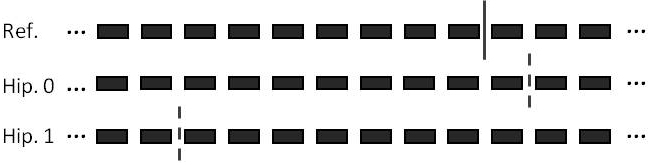
\includegraphics[width=0.47\textwidth]{windiffzoom.jpg}
	\caption{Exemplo de construção de uma matriz de rank}
	\label{fig:exemplomatrixrank}

  \end{figure}


  \begin{figure}[!h]

	\centering
	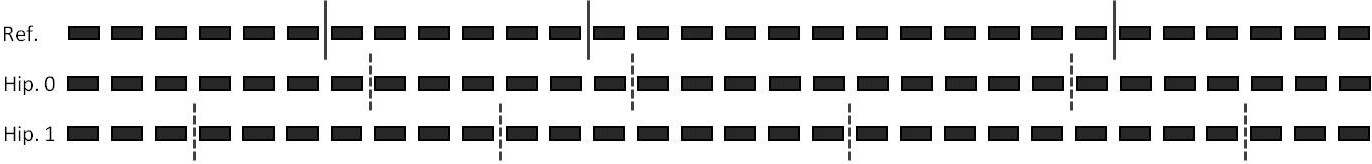
\includegraphics[width=0.47\textwidth]{windiff.jpg}
	\caption{Exemplo de construção de uma matriz de rank}
	\label{fig:exemplomatrixrank}

  \end{figure}



\subsubsection{Pk}

\subsubsection{WindowDiff}

Pevzner~\cite{Pevzner200219} aponta problemas na avaliação mais tradicional Pk~\cite{Beeferman1999}, como a demasiada penalização dos falsos negativos e a desconsideração de \textit{near misses}, quando um limite entre tópicos não casa exatamente com esperado mas fica próximo a ele.

A ideia é mover uma janela pelo texto e penalizar o algoritmo sempre que o número de limites (proposto pelo algoritmo) não coincidir com o número de limites (reais) para aquela janela de texto. % {Ctrl + C ???????}
